\newcommand{\ClassPath}{../../VIU_TFM_LaTeX_template}
\documentclass{\ClassPath/viu-tfm-template}
\usepackage{multicol}

\definecolor{maincolor}{HTML}{f25416}

%--------------------------------------------------------------------------
% Definiciones necesarias Modifica con tus datos
%--------------------------------------------------------------------------
\def\nombre{Gómez Olivencia, Rubén}
\def\dni{78910013-A}
\def\titulo{Juego del solitario creado con \linebreak\linebreak HTML, CSS y Javascript}
\def\titulacion{Máster Universitario en Desarrollo de Aplicaciones y Servicios Web}
\def\curso{2022-2023}

%Los siguientes son opcionales: si no se ponen, la portada cambia un poco. Ideal para escribir artículos/trabajos cortos
\def\dirige{}
\def\convocatoria{}
\def\asignatura{Desarrollo de aplicaciones web II: lado del cliente (front-end) y multimedia}


% importar fichero de Bibliografía
%\addbibresource{Actividad_1.bib}

\begin{document}
    \graphicspath{{../../VIU_TFM_LaTeX_template/}}

    \coverpage

    \tableofcontents

\chapter{Introducción}

A lo largo de este documento se van a explicar las decisiones tomadas, tanto en el ámbito de programación como de diseño, durante el desarrollo de un juego basado en el popular juego de cartas “el solitario”.

Para la realización de este juego se ha hecho uso del lenguaje de marcado de hipertexto \textbf{HTML}, junto con el sistema de hojas de estilo en casacada \textbf{CSS} y el lenguaje de programación \textbf{Javascript}.


\chapter{Arquitectura cliente-servidor}
A la hora de realizar una aplicación web, o como en este caso un juego, tenemos que tener en cuenta cómo funciona la arquitectura que hace posible que podamos interactuar con él.

Cuando navegamos por internet se hace uso de la conocida como arquitectura \textbf{Cliente - Servidor}, en la que podemos diferenciar, como su nombre indica, dos apartados:

\begin{itemize}
    \item \textbf{Servidor}: Un servidor es un ordenador potente que recibe peticiones, las procesa y devuelve una respuesta dependiendo de la petición recibida. En el caso de una aplicación web, el servidor contará con un servicio que recibirá peticiones \textbf{HTTP} y responderá con respuestas en código HTML, imágenes, ficheros ... Entre los servidores web más conocidos están: \href{https://httpd.apache.org/}{Apache HTTP Server}, \href{https://nginx.org/}{Nginx}, \href{https://www.iis.net/}{IIS}, ...

    \item \textbf{Cliente}: A la hora de interactuar con una aplicación web el cliente es quien va a realizar las peticiones al servidor. Normalmente el cliente es un navegador web utilizado por un usuario. Entre los navegadores web más conocidos están: \href{https://www.mozilla.org/es-ES/firefox/}{Firefox}, \href{https://www.google.com/chrome/}{Chrome}, \href{https://www.microsoft.com/es-es/edge}{Edge}, ...
\end{itemize}

A la hora de interactuar, un usuario hará uso del cliente (navegador web), con el que interactuará para realizar, normalmente, peticiones al servidor en busca de información. A continuación se puede ver un dibujo de cómo funciona la interacción descrita:


\begin{center}
    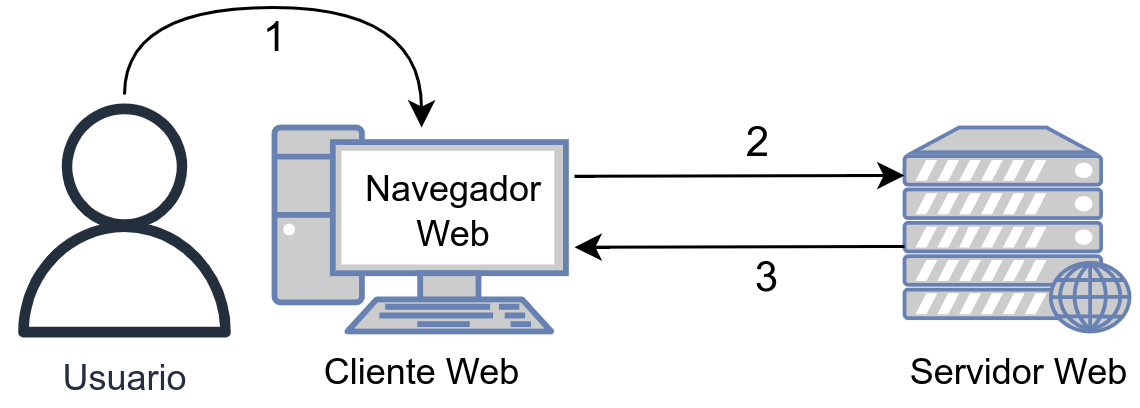
\includegraphics[width=0.6\linewidth]{img/cliente_servidor.png}
\end{center}

Tal como se puede ver en la imagen, los pasos que se realizan son:

\begin{enumerate}
    \item \textbf{Usuario interactúa con navegador web}. Tal como hemos dicho, un navegador web es el cliente de nuestra arquitectura, que es utilizado por el usuario. Cuando un usuario accede a una web, hace click en un enlace o realiza una búsqueda,  está comenzando el proceso del siguiente paso.

    \item \textbf{Realizar petición}. El navegador detecta lo que el usuario quiere realizar, y en ese momento lanza una petición (o varias) pidiendo al servidor web lo solicitado (una nueva web, una búsqueda, ...).

    \item \textbf{Devolver respuesta}: El servidor web recibe la petición, la procesa, y devuelve el resultado al cliente (navegador web) que mostrará por pantalla.
\end{enumerate}

\section{Backend vs. Frontend}
En la arquitectura mostrada previamente, a la hora de diseñar el software, entran en juego también dos partes, que se encargarán por separado de procesar la entrada y realizar una salida:

\begin{itemize}
    \item El \textbf{Back end} es el software que se ejecuta en la parte de \textbf{servidor}, que recibe las peticiones del cliente, las procesa (gestión de autenticación, acceder a base de datos, realizar cálculos, obtener información...) y que posteriormente el servidor devolverá.

    En este apartado de \textbf{backend} se hace uso de lenguajes de programación como \href{https://www.php.net/}{PHP} o \href{https://www.java.com/es/}{Java}, frameworks como \href{https://rubyonrails.org/}{Ruby on Rails}... , por poner sólo unos pocos.

    \item El \textbf{Front end} es la parte que se ejecuta en la parte \textbf{cliente} (navegador web) de la arquitectura anterior. Mostrará la información atendiendo al diseño recibido, teniendo en cuenta la información HTML y las hojas de estilos CSS.

    También existe la posibilidad de ejecutar código que alterará, o que nos permitirá interactuar con la web. Este código está escrito en lenguaje \textbf{javascript} y que se ejecuta enteramente en el lado cliente (navegador web).
\end{itemize}

El juego realizado, que se va a detallar a continuación, ha sido realizado para que pueda ser ejecutado enteramente en la parte \textbf{frontend}. Esto hace que no sea necesario un servidor con el que interactuar, y por tanto sólo el navegador web ejecutará todas las funciones necesarias para poder jugar.


\chapter{Normas del juego}

Aunque el juego del solitario es conocido, a continuación se va a detallar brevemente las normas del juego, ya que es importante para entender el desarrollo realizado.

Las reglas del juego son las siguientes:

\vspace{-1em}
\begin{itemize}
    \item La baraja de cartas consta de:
    \begin{itemize}
        \item 4 palos nombrados como “viu”,”cuadrados”, “hexágonos” y “círculos”. Los dos primeros tienen color naranja y los dos últimos color gris.
        \item Cada palo tiene 12 cartas numeradas del 1 al 12.
    \end{itemize}
    \item La mesa de juego contará con seis tapetes (donde se colocarán mazos de cartas).
    \item Los tapetes tienen las siguientes funciones:
    \begin{itemize}
        \item \textbf{Tapete inicial}: donde se sitúa el mazo completo ya barajado al inicio de la partida. Este tapete nunca podrá recibir cartas mientras haya cartas en él.
        \item \textbf{4 tapetes receptores}: donde se sitúan las cartas en orden decreciente (empezando siempre por una carta con el número 12) y alternando los colores. No se puede saltar ningún número y nunca podrán ir dos cartas del mismo color seguidas.
        \item \textbf{Tapete sobrantes/descartes}: donde se pondrán las cartas de manera temporal desde el tapete inicial ya que no es posible ponerlas sobre ningún tapete receptor.

        Es posible mover una carta de este tapete a uno receptor en cualquier momento.
    \end{itemize}

    \item Cuando no queden cartas en el tapete inicial, se cogerán las cartas del  tapete sobrantes, se barajarán y se pondrán sobre el tapete inicial.

    \item El juego termina cuando no haya ninguna carta sobre el tapete inicial ni el sobrantes.
\end{itemize}
\vspace{-1em}

La mesa de juego tiene la siguiente forma, donde se pueden ver los distintos tapetes, en la fila superior el inicial (más grande) y el sobrantes, y abajo los cuatro de recepción:
\begin{center}
    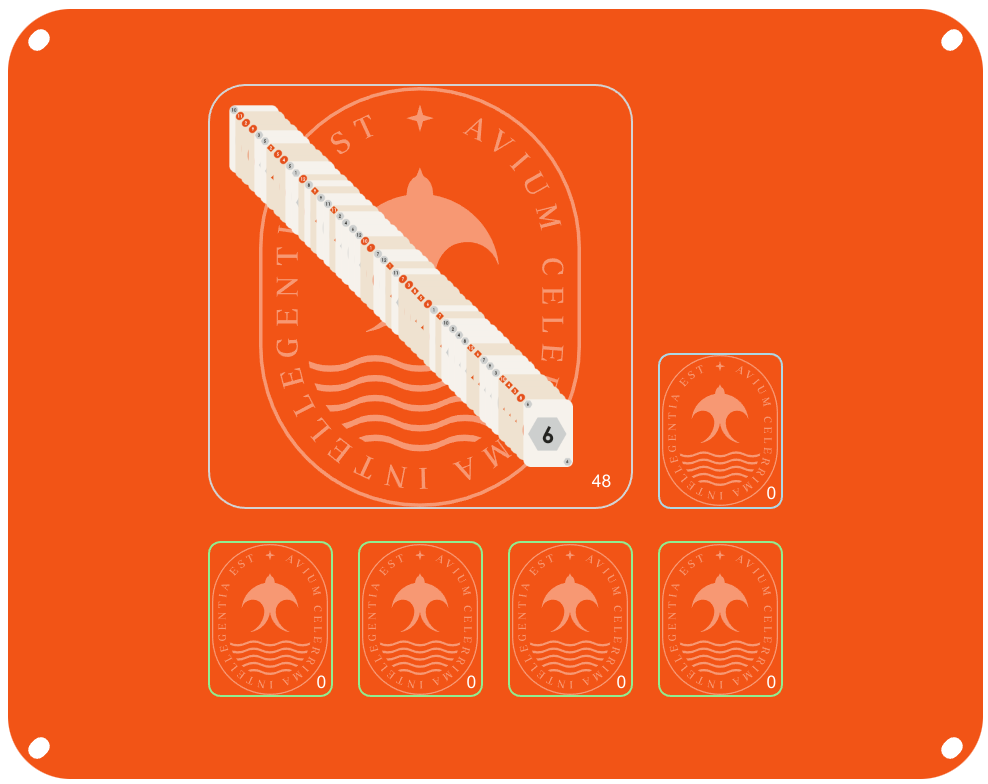
\includegraphics[width=0.7\linewidth]{img/mesa.png}
\end{center}


\chapter{Desarrollo realizado}

Teniendo en cuenta las reglas previas, se ha tenido que realizar el desarrollo siguiendo dichos criterios. En este apartado no se va a detallar el aspecto visual del mismo, y nos vamos a centrar en la parte programada en \textbf{javascript}.

A la hora de realizar el desarrollo existen distintos aspectos y etapas que tiene el juego. A continuación se exponen y serán detallados más adelante:

\begin{itemize}
    \item Variables globales
    \item Comienzo del juego
    \begin{itemize}
        \item Barajar y cargar el tapete inicial
        \item Control del tiempo y contadores
    \end{itemize}
    \item Mover carta entre tapetes
    \item Fin del juego
\end{itemize}
\vspace{-1em}


\section{Variables globales}
A la hora de realizar el juego se han creado distintas variables globales que pueden ser accedidas desde cualquier parte del juego. Esto facilita el realizar cambios en los valores de las mismas.

Sin entrar en las variables de los palos y los números, existen tres variables globales principales que son las siguientes:

\vspace{-1em}
\begin{itemize}
    \item \textbf{Tapetes}: Los tapetes existentes en el juego, que son los objetos DOM del HTML.

\begin{mycode}{Variable para los tapetes, con el DOM correspondiente}{javascript}{}
// Tapetes
let tapetes = [
    document.getElementById("inicial"),
    document.getElementById("receptor1"),
    document.getElementById("receptor2"),
    document.getElementById("receptor3"),
    document.getElementById("receptor4"),
    document.getElementById("sobrantes")
]
\end{mycode}


    \item \textbf{Mazos}: Los mazos que habrá durante el juego, cada uno encima de un tapete distinto.
\begin{mycode}{Variable para los mazos}{javascript}{}
// Mazos
let mazos = [
    [], // inicial
    [], // receptor1
    [], // receptor2
    [], // receptor3
    [], // receptor4
    [], // sobrantes
]
\end{mycode}
    \item \textbf{Contadores}: Los contadores que controlan cuántas cartas hay en cada tapete. También son elementos del DOM para poder ser actualizados.
\end{itemize}
\vspace{-1em}


Cada una de estas tres variables son un array de seis posiciones, siguiendo el orden:

\vspace{-1em}
\begin{itemize}
    \item \textbf{Inicial}: Tiene que ver con el tapete/mazo inicial. Posición cero del array.
    \item \textbf{Tapetes receptores}: Hay cuatro tapetes receptores, y por tanto cuatro posiciones en el array para cada uno de ellos (1..4).
    \item \textbf{Sobrante}: La última posición (5) es para el tapete sobrante, su mazo y el contador del mismo.
\end{itemize}
\vspace{-1em}

\section{Comienzo del juego}
Tal como se ha podido ver previamente, el comienzo del juego se ha diferenciado en dos apartados, que se realizan de manera consecutiva.

Para que comience el juego, primero debemos hacer click sobre el botón situado en la parte inferior con el aspecto:

\vspace{-1.6em}
\begin{center}
    
\includegraphics[width=0.2\linewidth]{img/boton.png}
\end{center}
\vspace{-1em}

Lo que llamará a la función \textbf{comenzar\_juego}:

\begin{mycode}{Evento onclick del botón para comenzar el juego}{javascript}{}
document.getElementById("reset").onclick = comenzar_juego;
\end{mycode}


\subsection{Barajar y cargar el tapete inicial}
Este apartado es el principal del juego, ya que se encarga de crear el mazo inicial  juntando las cartas de cada uno de los palos de la baraja.

Para ello se recorren los palos y las cartas y se añaden al array de mazos (posición “0”, para el mazo inicial). Se crean objetos imágenes, indicando cuál es el origen de la imagen a utilizar, indicamos que los objetos se pueden mover (“\textit{draggable}”) y añadimos ciertos atributos que después necesitaremos para aceptar o denegar el movimiento entre tapetes.

Este mazo inicial se baraja en la función \textbf{barajar}, que recibe el mazo como parámetro, que también se utilizará al pasar las cartas del tapete sobrantes al inicial.

Y por último, se colocan las cartas sobre el tapete inicial a través de la función \textbf{cargar\_tapete\_inicial} haciendo un efecto en cascada diagonal.


\subsection{Control del tiempo y contadores}
Este apartado no es estrictamente necesario para el juego, pero da valor a la hora de que sea más ameno si queremos tratar de batir nuestro propio récord, ya sea de tardar menos o realizar el menor número de movimientos posibles.

El juego cuenta con un control de tiempo, que es un \textit{interval} que se llama cada segundo, realizando un incremento de tiempo para posteriormente ser visualizado en el formato “HH:MM:SS” (donde “HH” son horas, “MM” minutos y “SS” segundos).

Existe un contador para cada tapete, situado en su esquina inferior derecha, para que el usuario sepa cuántas cartas tiene el mazo que está sobre él.

Y por último, existe el contador de movimientos, que se incrementa cada vez que movemos una carta sobre cada uno de los tapetes.

Tanto el tiempo como el contador de movimientos se puede ver en la parte superior de la página, encima de la mesa de juego:

\vspace{-1em}
\begin{center}
    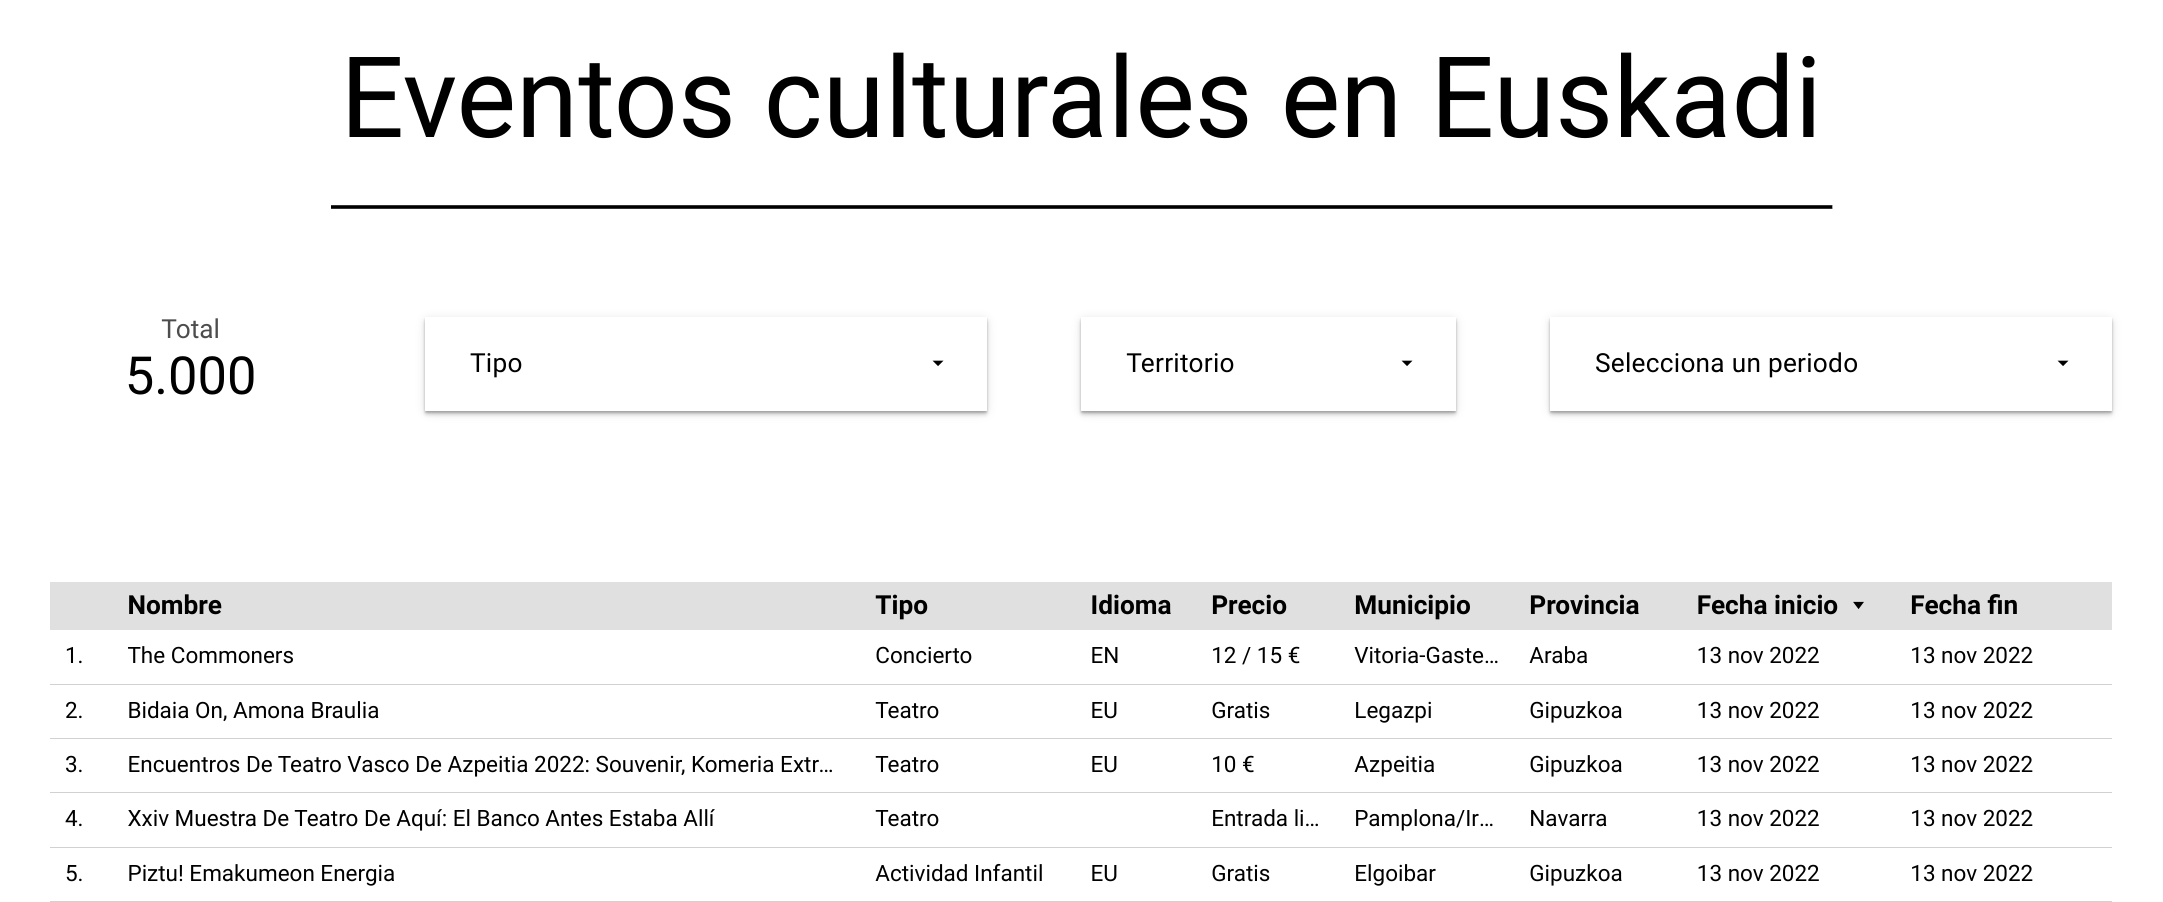
\includegraphics[frame,width=0.8\linewidth]{img/cabecera.png}
\end{center}
\vspace{-1em}

Tras esto, el botón que daba comienzo al juego se ha cambiado de color y ahora pone “Reiniciar”, lo que reiniciará el juego, limpiando tapetes, contadores, volviendo a barajar y situando las cartas de nuevo en el tapete inicial.

\vspace{-1.6em}
\begin{center}
    
\includegraphics[width=0.2\linewidth]{img/reiniciar.png}
\end{center}
\vspace{-1em}


\subsection{Mover carta entre tapetes}
Este es el apartado más importante dentro de la programación del juego, ya que contiene la lógica de lo que se debe realizar al tratar de mover una carta entre tapetes.

Toda esta funcionalidad está basada en la API \textit{Drag and Drop} añadida en el primer borrador de HTML5 en el \href{https://www.w3.org/TR/2008/WD-html5-20080122/#dnd}{2008}, que nos permite arrastrar y soltar elementos de la web generando un evento.

A continuación se detallan cuáles son los pasos que se realizan en esta funcionalidad:

\vspace{-1em}
\begin{enumerate}
    \item \textbf{Al mover carta}: Hay que tener en cuenta que sólo se puede mover la carta que está más arriba del montón del tapete inicial y del tapete sobrantes, quedando el resto “bloqueadas” (incluidas las de los tapetes receptores).

    Al intentar mover una de estas cartas superiores, se lanza el evento y se obtiene información de la carta y del mazo origen.

    \item \textbf{Soltar carta}: Este es el momento en el que la carta se suelta sobre uno de los tapetes receptores o sobrantes. El tapete inicial no permite que se suelten cartas sobre él.

    Si se mueve la carta sobre el tapete de sobrantes, no hay que realizar ninguna comprobación, por lo que se pasa al siguiente paso.

    En cambio, si se intenta soltar sobre un tapete receptor, hay que comprobar lo siguiente:
        \begin{itemize}
            \item Si no hay cartas en el tapete, sólo se permite soltar una carta con el número 12.
            \item Si hay alguna carta sobre el tapete, la carta que se suelte encima tiene que ser de una única unidad inferior y de color distinto.
        \end{itemize}
    Si cualquiera de estas dos opciones no es válida, la carta vuelve al tapete de origen. A continuación parte de la función \textbf{soltar\_carta}:
\end{enumerate}
\vspace{-0.5em}

\begin{mycode}{Controlamos si la carta se puede soltar}{javascript}{{\footnotesize }}
if (mazo_receptor.length == 0 && numero == 12){
  // es una carta con número 12 y va a ser la primera carta del tapete
  carta.draggable = false;
  // movemos la carta de un mazo a otro
  mover_carta(mazo_origen,mazo_receptor,tapete_receptor,cont_origen,cont_receptor);
} else if (mazo_receptor.length != 0) {
  // no es la primera carta del tapete. Tenemos que ver
  // el número de la carta que ya está en ese tapete y su color.
  carta_mazo_num = mazo_receptor[mazo_receptor.length-1].getAttribute("data-numero");
  carta_mazo_col = mazo_receptor[mazo_receptor.length-1].getAttribute("data-color");
  if (carta_mazo_num-1 == numero && carta_mazo_col != color ) {
    // aceptamos la carta porque el número es uno menos que la que ya está
    // y es de distinto color/palo
    carta.draggable = false;
    mover_carta(mazo_origen,mazo_receptor,tapete_receptor,cont_origen,cont_receptor);
    }
}
\end{mycode}

\vspace{-1em}
\begin{enumerate}
    \item[3.] \textbf{Mover carta}: Si las comprobaciones del paso anterior son correctas, la carta se mueve al nuevo tapete. Tal como se puede ver en el código anterior, existe la función \textbf{mover\_carta} que recibe varios parámetros.

    En esta función también se actualizan los \textbf{contadores} llamando a otras funcione para restar o incrementar el contador, según sea el caso.
\end{enumerate}
\vspace{-1em}

Hay que recordar que cuando se mueve la última carta del tapete inicial (ya sea sobre uno de los tapetes receptores o el de sobrantes) se cogerán todas las cartas del tapete sobrantes, se barajarán de nuevo y se colocarán en el tapete inicial para continuar la partida.

Para limpiar el tapete correspondiente, lo que tenemos que hacer es eliminar los nodos hijos que son “img”, y para ello se ha creado una función:
\begin{mycode}{Controlamos si la carta se puede soltar}{javascript}{}
// función para limpiar el tapete de cartas
function limpiar_tapete(tapete) {
    while (tapete.getElementsByTagName('img').length>0) {
        tapete.getElementsByTagName('img')[0].remove();
    }
}
\end{mycode}



\subsection{Fin del juego}
La comprobación de ver si el juego ha finalizado se realiza cada vez que se mueve una carta de manera correcta.

Esta comprobación es sencilla, y lo que hace es comprobar que el contador del tapete inicial y el de sobrantes es igual a cero. En este caso el juego se da por terminado.

A la hora de finalizar el juego se para el contador, las cartas realizarán un efecto que se desplazan por la mesa de juego, para poder ver todas ellas:

\vspace{-1em}
\begin{center}
    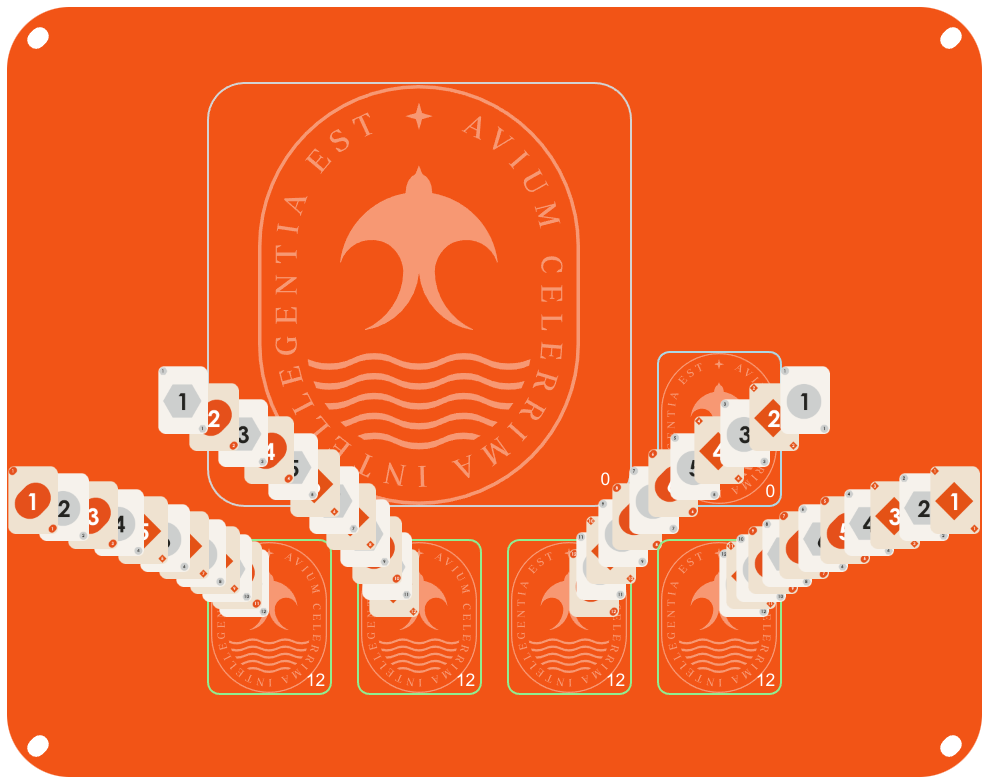
\includegraphics[width=0.8\linewidth]{img/final.png}
\end{center}
\vspace{-1em}

Y nos saldrá un aviso con el número de movimientos realizados, junto con tiempo empleado y preguntando al usuario si quiere volver a jugar:

\vspace{-1em}
\begin{center}
    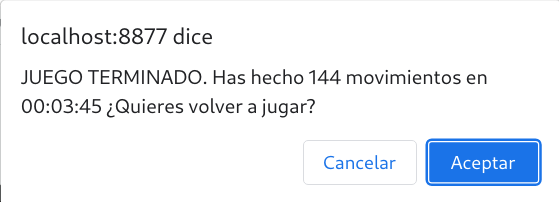
\includegraphics[frame,width=0.3\linewidth]{img/aviso.png}
\end{center}
\vspace{-1em}

En caso de aceptar el aviso, el juego se reiniciará. En caso de cancelar, podremos ver cómo ha quedado el tapete, el tiempo y el número de movimientos. En todo caso, podremos volver a reiniciar el juego con el botón de “Reiniciar”.

\chapter{Aspecto visual}
Para mejorar el aspecto visual del juego, se han realizado unas pequeñas modificaciones en la plantilla propuesta para el juego:

\vspace{-1em}
\begin{itemize}
    \item \textbf{Colores corporativos}: El tapete se ha modificado para que cuente con el color corporativo de la VIU, haciendo uso de una variable dentro del CSS.
    \begin{mycode}{Variable global en CSS para el color}{css}{}
/* Variable global de color */
:root {
    --corporativo: #F25416;
}
\end{mycode}

    \item \textbf{Redondear tapetes}: Gracias a la funcionalidad “border-radius” de CSS se ha hecho que los tapetes tengan un aspecto más redondeados en lugar de cuadrados.

    \item \textbf{Personalizar tapetes}: Para personalizar la mesa de juego, se ha añadido el sello de la VIU a cada uno de los tapetes, que junto con el borde, hace que se vea más claramente dónde se pueden colocar las cartas.

    \vspace{-0.6em}
    \begin{center}
        
\includegraphics[frame,width=0.26\linewidth]{img/tapete.png}
    \end{center}
    \vspace{-2em}

    \item \textbf{Borde de la mesa}: Se ha añadido un borde, que sólo aparece en las esquinas de la mesa de juego, con el fondo del logotipo de la VIU en color blanco.

    \item \textbf{Uso de Bootstrap}: Se ha hecho uso del sistema \textit{grid} de Bootstrap para dar tamaño a la mesa y colocar el temporizador y el contador de movimientos.
\end{itemize}
\vspace{-1em}


\chapter{Dificultades del proyecto}

Como todo proyecto de programación, durante el desarrollo nos podemos encontrar con ciertas dificultades que deben ser subsanadas para llegar a cumplir los requisitos planteados al comienzo del proyecto.

En este caso, la lógica del juego hace que sea un desarrollo sencillo, en el que no hay que tener demasiadas cosas en cuenta, por lo que la lógica del juego es sencilla.

Ahora bien, eso no quita que haya habido dificultades al realizar el proyecto, ya que se han usado ciertos aspectos nunca vistos previamente por el programador, que son:

\begin{itemize}
    \item \textbf{API drag and drop}: Aunque la mecánica de la API de HTML5 es sencilla, se ha tenido que profundizar en cómo funcionan las distintos funciones que se pueden utilizar en la API. Con ello, también se ha investigado la información que se puede enviar a través de los eventos generados en cada una de esas funciones.

    Las funciones de la API utilizadas han sido “\textbf{ondragstart}”, al comenzar el movimiento de la carta, y “\textbf{ondrop}”, para cuando se suelta sobre un tapete. Otras de las funciones existentes en la API (“onstart”, “ondragend”, “ondragleave”) no han sido necesarias, pero se han inicializado para que no hagan nada.

    \item \textbf{Colocación de las cartas}: Debido a la flexibilidad de CSS, y la colocación de imágenes teniendo en cuenta su posición relativa respecto al contenedor, ha sido necesario entender cómo funciona los estilos “float”, “position”, sobre todo para el efecto final.

    \item \textbf{Intervalos}: Aunque ya habían sido utilizados por parte del programador, debido a que no los utiliza de manera habitual, ha sido interesante recordar su funcionalidad.

    \item \textbf{Promesas}: Igual que el caso anterior, aunque se conocía el uso de “\textit{Promise}” para realizar \textbf{programación asíncrona}, se ha hecho uso de ellas para el efecto final de movimiento de las cartas. De esta manera se realiza una pequeña pausa al mover cada una de las cartas, y hay que esperar para que salga el aviso de finalización del juego.
\end{itemize}


\chapter{Conclusiones}

A la hora de afrontar un proyecto, aunque el algoritmo generado sea sencillo, no quita que exista un proceso de aprendizaje a la hora de utilizar ciertas herramientas no conocidas.

Este ha sido el caso durante la programación en \textbf{Javascript} y el uso de ciertas funcionalidades de \textbf{HTML5} y \textbf{CSS} versión 3 no conocidas hasta ahora.

Esto nos va a permitir que las aplicaciones generadas para el lado del cliente (conocido como programación \textbf{frontend}) tengan más funcionalidades y de esta manera podamos realizar aplicaciones más complejas.


%\printbibliography[title={Referencias bibliográficas},heading=bibintoc]

\end{document}
